\documentclass[
]{jss}

\usepackage[utf8]{inputenc}

\providecommand{\tightlist}{%
  \setlength{\itemsep}{0pt}\setlength{\parskip}{0pt}}

\author{
Stephanie Kobakian\\Queensland University of Technology \And Dianne Cook\\Monash University \And Earl Duncan\\Queensland University of Technology
}
\title{An Algorithm For Spatial Mapping Using a Hexagon Tile Map, With
Application to Australian Maps}

\Plainauthor{Stephanie Kobakian, Dianne Cook, Earl Duncan}
\Plaintitle{An Algorithm For Spatial Mapping Using a Hexagon Tile Map, With
Application to Australian Maps}
\Shorttitle{An Algorithm For Spatial Mapping Using a Hexagon Tile Map}

\Abstract{
This algorithm creates a tesselated hexagon display to represent each of
the spatial polygons. It allocates these hexagon in a manner that
preserves the spatial relationship of the geographic units. It showcases
spatial distributions, by emphasising the small geographical regions
that are often difficult to locate on geographic maps. Spatial
distributions have been presented on alternative representations of
geography for many years. In modern times, interactivity and animation
have begun to play a larger role, as alternative representations have
been popularised by online news sites, and atlas websites with a focus
on public consumption. Applications are increasingly widespread,
especially in the areas of disease mapping, and election results.
}

\Keywords{spatial, statistics, cartogram}

%% publication information
%% \Volume{50}
%% \Issue{9}
%% \Month{June}
%% \Year{2012}
%% \Submitdate{}
%% \Acceptdate{2012-06-04}

\Address{
    Stephanie Kobakian\\
  Queensland University of Technology\\
  School of Mathematical Sciences, Science and Engineering Faculty,
  Brisbane, QLD, Australia\\
  E-mail: \email{stephanie.kobakian@qut.edu.au}\\
  
      Dianne Cook\\
  Monash University\\
  Department of Econometrics and Business Statistics, Melbourne, VIC,
  Australia\\
  E-mail: \email{dicook@monash.edu}\\
  
      Earl Duncan\\
  Queensland University of Technology\\
  School of Mathematical Sciences, Science and Engineering Faculty,
  Brisbane, QLD, Australia\\
  E-mail: \email{earl.duncan@qut.edu.au}\\
  
  }


% Pandoc header

\usepackage{amsmath}

\begin{document}

\setcounter{page}{65}

\hypertarget{introduction}{%
\section{Introduction}\label{introduction}}

The current practice for presenting geospatial data is a choropleth map
display. These maps highlight the geographic patterns in geospatially
related statistics \citep{SAMGIS}. The land on the map space is divided
into geographic units, these boundaries are usually administrative, such
as states or counties. The units are filled with colour to represent the
value of the statistic \citep{EI}.

Australian residents are increasingly congregating around major cities,
the vast rural areas are often sparsely populated in comparison to the
urban centres. In Australia, government bodies such as the Australian
Bureau of Statistics (ABS), and the Australian Electoral Commission
(AEC) hold the responsibility for the division of the population into
geographic units. If it necessary, the AEC may adjust the boundaries of
the areas as the population increases. The division of the population
into approximately equal population areas results in dramatically
different square meterage of the geographic areas. This can give unequal
attention to the statistic of each area, this can cause
misrepresentation of the spatial distributions of human related
statistics in geographic maps.

The solutions to this visualisation problem begin with the geography.
Cartograms apply a transformation to the geographic boundaries based on
the value of the statistic of interest. These displays result in a
distortion of the map space to represent differences in the statistic
across the areas \citep{ACCAC}. The statistic of interest is used to
determine the cartogram layout. When the Australian population is the
statistic of interest, the result is a population cartogram. They fail
to preserve a recognisable display due to the difference in size of
metropolitan and rural areas \citep{ACTUC}, \citep{GOINO}. Contiguous
cartograms change the shape of areas, while preserving boundary
relationships of neighbours. Non-contiguous cartograms maintain the
geographic shape of each geographic area, but will lose the connection
to neighbours as the polygon for each geographic area shrinks or grows.

Alternative maps shift the focus from land area and shape, to the value
of the statistics in a group of areas. Alternative mapping methods allow
increased understanding of the spatial distribution of a variable across
the population, by fairly representing each administrative area. This
acknowledges that the amount of residents can be different but
recognises that each area, or person within it is equally important.

tile maps, Rectangular cartograms \citep{ORC} and Dorling cartograms
\citep{ACTUC}, all use one simple shape to represent each area. They
place various importance on the preservation of spatial relationships,
but all decrease the emphasis on the size of the geographic areas. These
alternative map displays focus on the relationship between neighbours,
attempting to preserve connections, and disregard the unique shapes of
the administrative boundaries.

The \pkg{sugarbag} package provides a new algorithm to create tesselated
hexagon tile maps. It emphasises the capital cities as population hubs,
and emphasises the distances rather than size of large, rural geographic
units.

\hypertarget{algorithm}{%
\section{Algorithm}\label{algorithm}}

The algorithm presented in \pkg{sugarbag} package operates on a set of
simple feature geometry objects, also known as \pkg{sf} \citep{sf}
polygons.

There are four steps performed to create a tesselated hexagon tile map.
These steps can be executed by the main function, \code{create_hexmap},
or can be implemented separately for more flexibility. There are
parameters used in the process that can be provided by users, if they
are not, they will be automatically derived.

\begin{enumerate}
\def\labelenumi{\arabic{enumi}.}
\tightlist
\item
  Create the set of centroids to allocate
\item
  Create the grid of hexagons locations to use
\item
  Allocate each centroid to an available hexagon
\item
  Transform the data for plotting
\end{enumerate}

\hypertarget{parameters}{%
\subsection{Parameters}\label{parameters}}

The \code{create_hexmap} function requires several parameters, if they
are not provided, the information will be derived from the simple
features (\pkg{sf}) set of shapes used. Users may choose to only use the
\code{allocate} function when they wish to use a set of centroids,
rather than \pkg{sf} polygons.

The following parameters must be provided to \code{create_hexmap}:

\begin{itemize}
\tightlist
\item
  \emph{shp:} an sf object containing the polygon information
\item
  \emph{sf\_id:} name of a column that distinguishes unique areas
\item
  \emph{focal\_points:} a data frame of reference locations used to
  allocate hexagons
\end{itemize}

\hypertarget{polygon-set}{%
\subsection{Polygon set}\label{polygon-set}}

The polygon set of Statistical Areas at Level 2 (SA2) \citep{abs2016} of
Tasmania in 2016 is provided with the \pkg{sugarbag} package as
\code{tas_sa2}. A single column of the data set is used to identify the
unique areas. In this case, the unique SA2 names for each SA2 have been
used.

The longitude and latitude centre of the capital cities of Australia are
used as focal points to allocate each geographic area around the closest
capital city. Hobart will be the common focal point, as this example
uses only the areas in the state of Tasmania.

\begin{CodeChunk}

\begin{CodeInput}
R> data(capital_cities)
\end{CodeInput}
\end{CodeChunk}

The following parameters will be determined within \code{create_hexmap}
if they are not provided. They are created as they are needed throughout
the following example:

\begin{itemize}
\tightlist
\item
  \emph{buffer\_dist:} a float value for distance in degrees to extend
  beyond the geometry provided
\item
  \emph{hex\_size:} a float value in degrees for the diameter of the
  hexagons
\item
  \emph{hex\_filter:} amount of hexagons around centroid to consider for
  allocation
\item
  \emph{width:} the angle used to filter the grid points around a
  centroid
\end{itemize}

\hypertarget{create-the-set-of-centroid-points}{%
\subsection{Create the set of centroid
points}\label{create-the-set-of-centroid-points}}

A set of centroids may be used directly. The set of polygons should be
provided as an \pkg{sf} object, this is a data frame containing a
\code{geometry} column. The \code{read_shape} function can assist in
creating this object for use in \texttt{R}.

The centroids can be derived from the set of polygons using the
\code{create_centroids} function:

\begin{CodeChunk}

\begin{CodeInput}
R> centroids <- create_centroids(shp_sf = tas_sa2, sf_id = "SA2_NAME16")
\end{CodeInput}
\end{CodeChunk}

\hypertarget{create-the-hexagon-grid-points}{%
\subsection{Create the hexagon grid
points}\label{create-the-hexagon-grid-points}}

A grid is created to ensure tessellation between the hexagons that
represent the geographic units on a hexagon tile map.

The grid of possible hexagon locations is made using the
\code{create_grid} function. It uses the centroids, the hexagon size and
the buffer distance.

\begin{CodeChunk}

\begin{CodeInput}
R> grid <- create_grid(centroids = centroids, hex_size = 0.2, buffer_dist = 1.2)
\end{CodeInput}
\end{CodeChunk}

\hypertarget{step-1-creating-a-tesselated-grid}{%
\subsubsection{Step 1: Creating a tesselated
grid}\label{step-1-creating-a-tesselated-grid}}

A set of longitude columns, and latitude rows are created to define the
locations of the hexagons. The distance between each row and column is
the size specified by \code{hex_size}. Equally spaced columns are
created from the minimum longitude minus the buffer distance, up to the
maximum longitude plus the buffer distance. Similarly, the rows are
created from the latitude values and the buffer distance. A unique
hexagon location is created from all intersections of the longitude
columns and latitude rows. Figure \ref{fig:grid2} shows the original
grid on the left, to allow for tessellating hexagons, every second
latitude row on the grid is shifted right, by half of the hexagon size.
The grid for tessellation is shown on the right.

\begin{CodeChunk}
\begin{figure}

{\centering 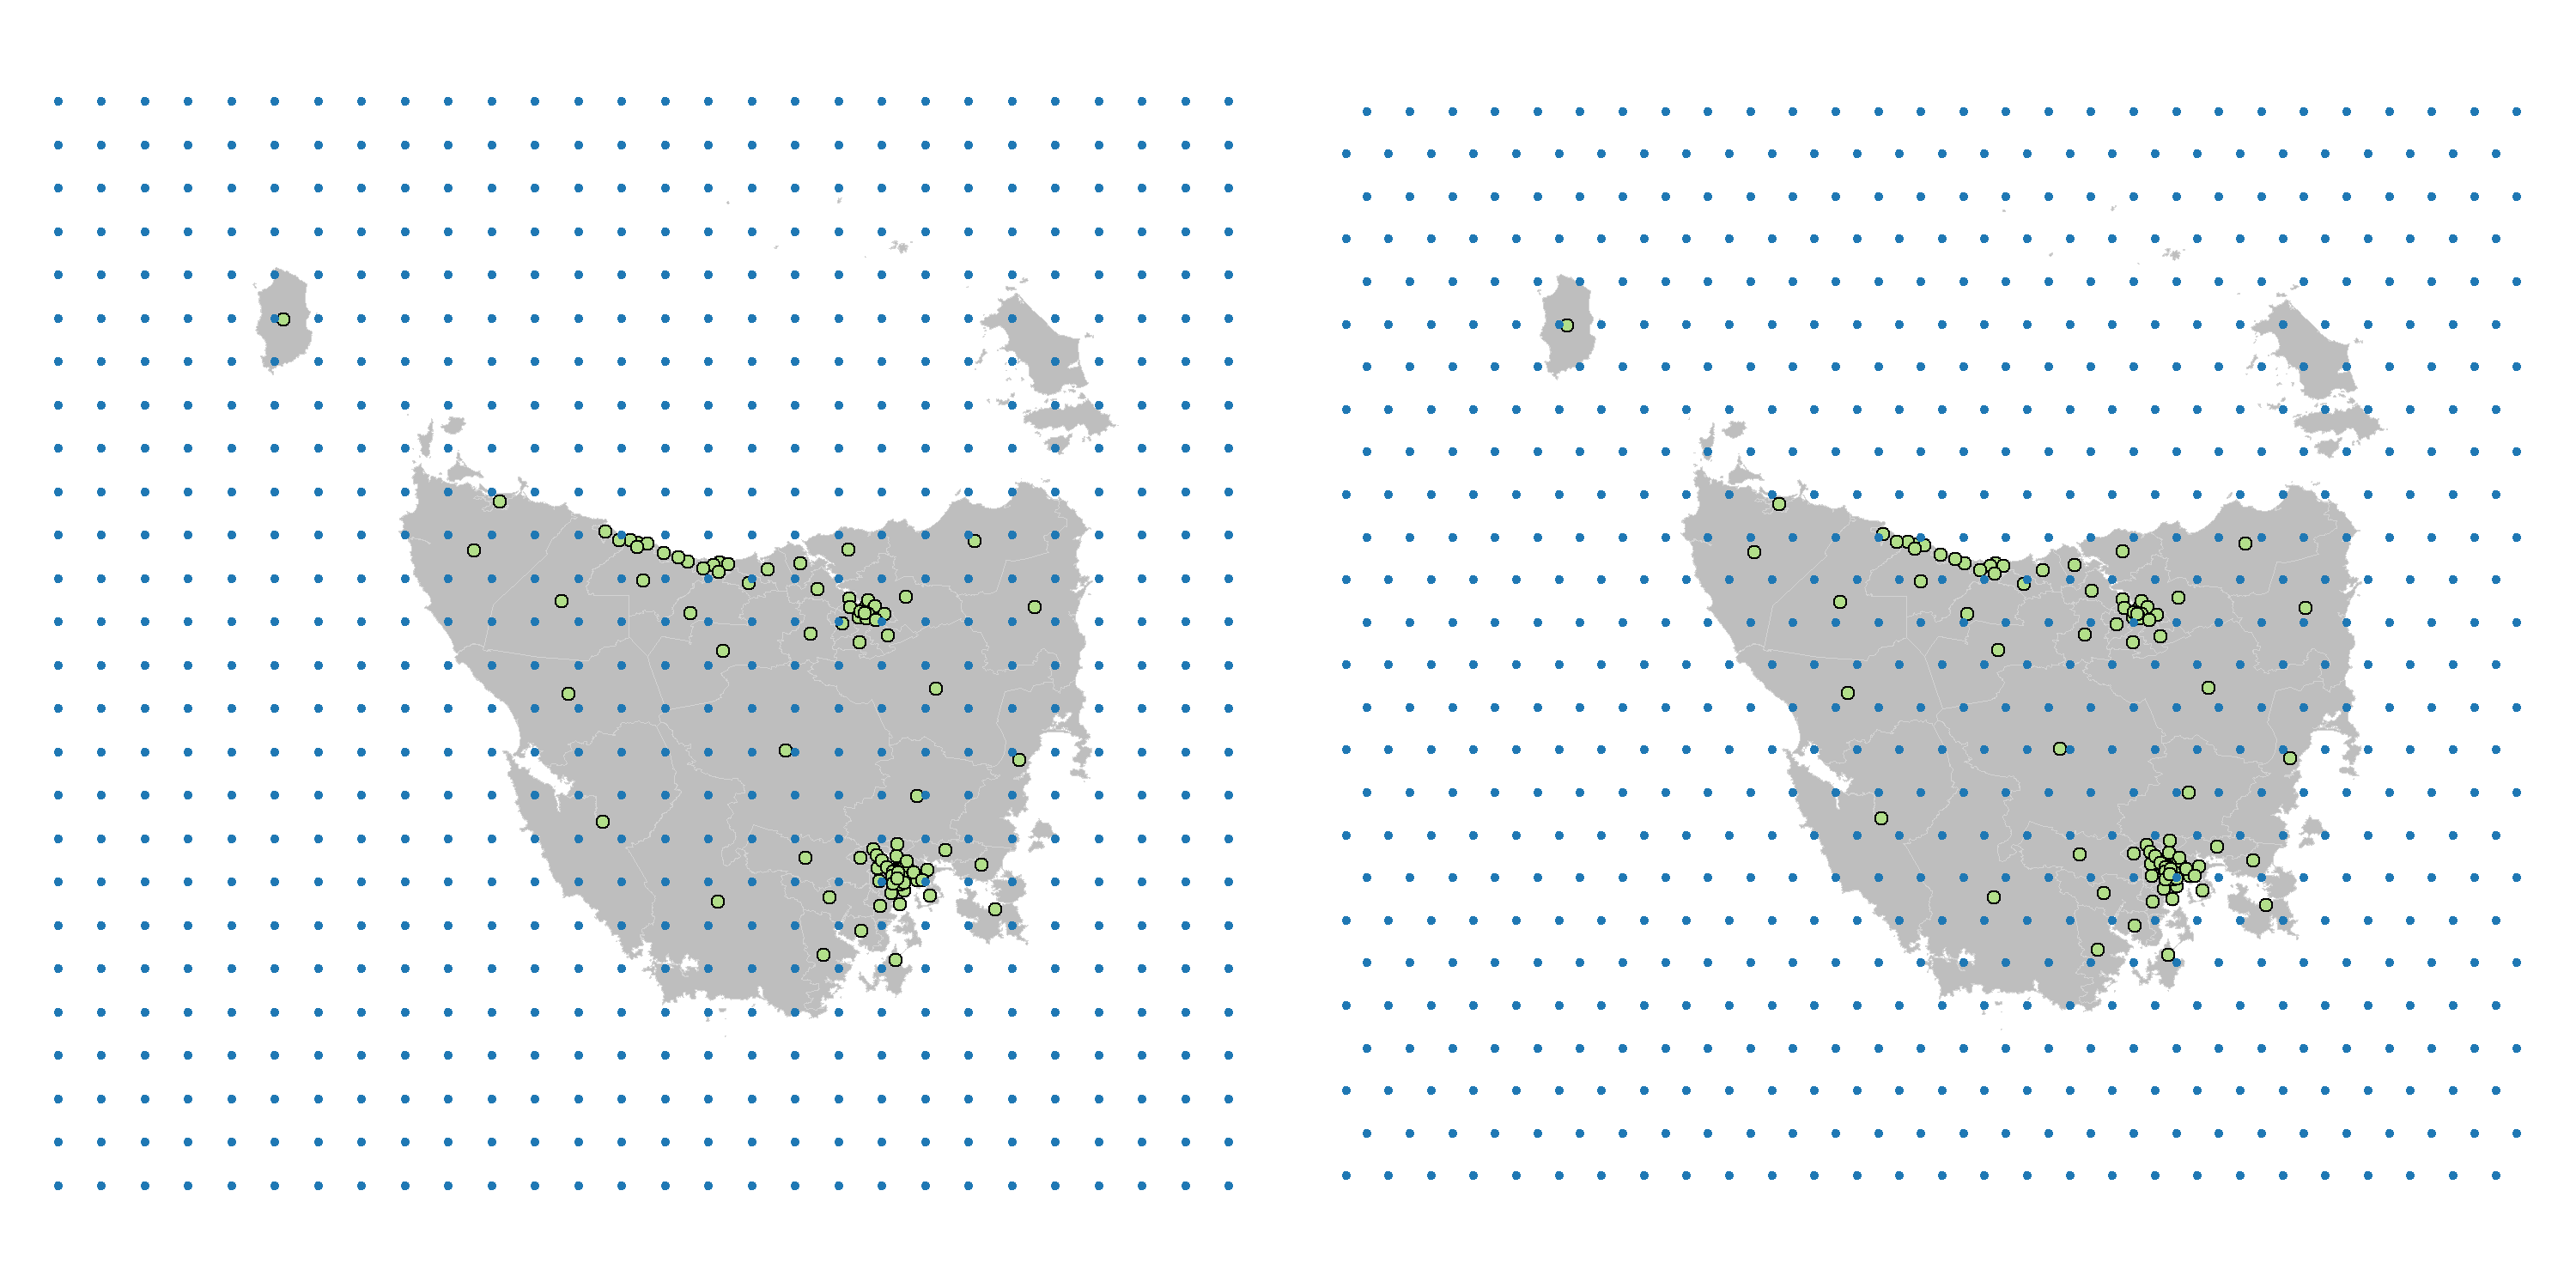
\includegraphics[width=1\linewidth]{figures/2grid} 

}

\caption[Grid points to create a tile map]{Grid points to create a tile map.}\label{fig:grid2}
\end{figure}
\end{CodeChunk}

\hypertarget{step-2-rolling-windows}{%
\subsubsection{Step 2: Rolling windows}\label{step-2-rolling-windows}}

Not all of the grid points will be used, especially if islands result in
a large grid space. To filter the grid for appropriate hexagon locations
for allocation, the \code{create_buffer} function is used by
\code{create_grid}. It finds the grid points needed to best capture the
set of centroids on a hexagon tile map.

The closest latitude row and longitude column are found for each
centroid location. Then rows and columns of centroids are divided into
20 groups. The amount of rows in each latitude group and the amount of
columns in each longitude group are used as the width of rolling
windows. The rolling windows can be seen on the bottom and right of the
gris shown in Fig. \ref{fig:filter_grid}. This will tailor the available
grid points to those most likely to be used. It also helps reduce the
amount of time taken, as it decreases the amount of points considered
for each centroid allocation.

The first rolling window function finds the minimum and maximum centroid
values for the sliding window groups of longitude columns and the groups
of latitude rows.

The second rolling window function finds the average of the rolling
minimum and maximum centroid values, for the longitude columns and
latitude rows.

\hypertarget{step-3-filtering-the-grid}{%
\subsubsection{Step 3: Filtering the
grid}\label{step-3-filtering-the-grid}}

The grid points are kept only if they fall between the rolling average
of the minimum and maximum centroid values after accounting for the
buffer distance, for each row and column of the grid. The sparsely
populated South-West region of National Park has much fewer points
available compared to the South-East region containing the city of
Hobart.

\begin{CodeChunk}
\begin{figure}

{\centering 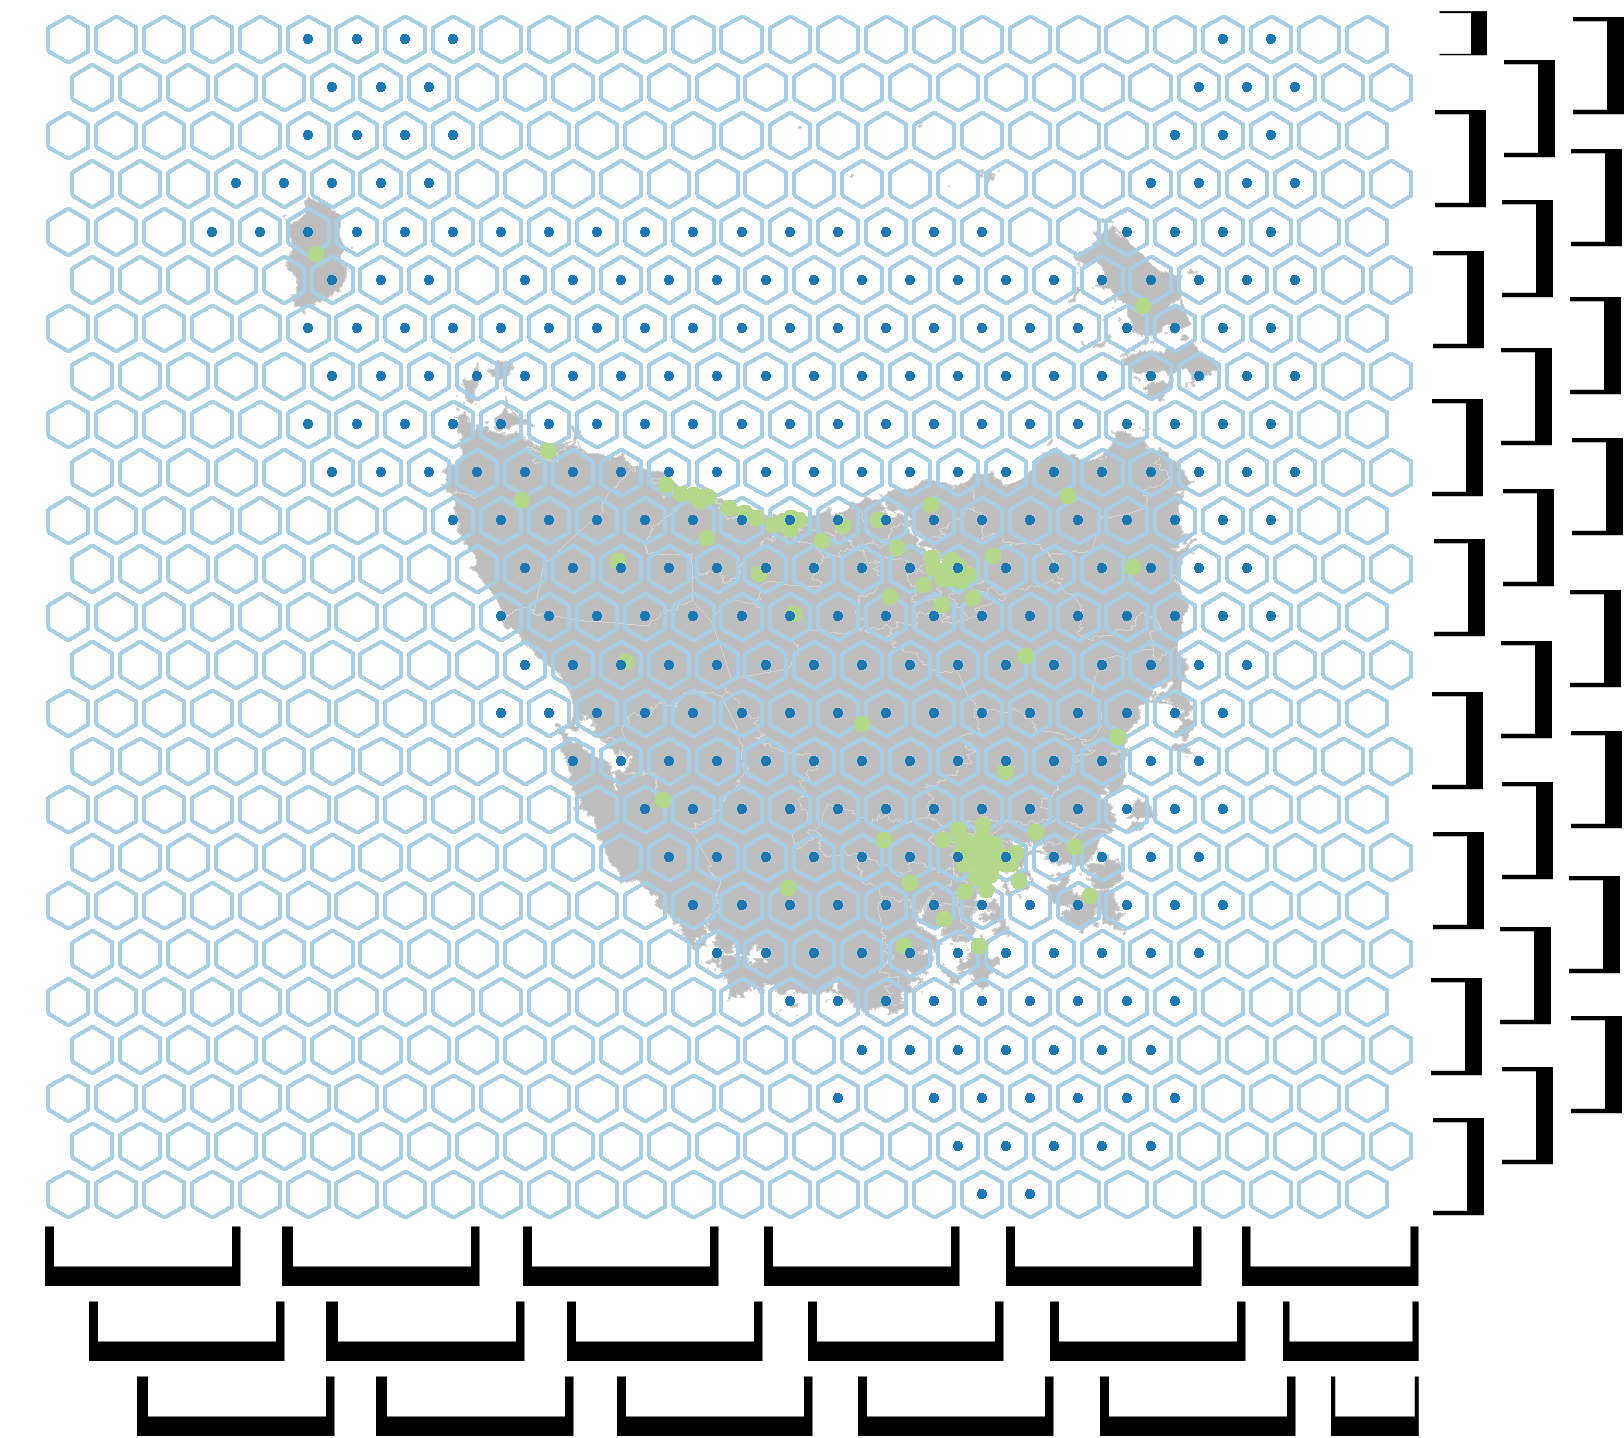
\includegraphics[width=1\linewidth]{figures/3grid} 

}

\caption[All possible hexagon locations from the initial grid are shown with blue outlines]{All possible hexagon locations from the initial grid are shown with blue outlines. The blue dots show the grid points left to choose from after the buffer step. The rolling windows show the collections of rows and columns used to filter the hexagon locations.}\label{fig:filter_grid}
\end{figure}
\end{CodeChunk}

\hypertarget{centroid-to-focal-point-distance}{%
\subsection{Centroid to focal point
distance}\label{centroid-to-focal-point-distance}}

The distance between each centroid in the set, and each of the focal
points provided is calculated. The name of the closest focal point, and
the distance and angle from focal point to polygon centroid is joined to
polygon data set. To minimise time taken for this step only one option
is provided, Tasmania's capital city Hobart. The order for allocation is
determined by the distance between the polygon centroid and it's closest
focal point. The points are arranged from the centroid closest to the
focal point(s), to the furthest.

\hypertarget{allocate-each-centroid-to-a-hexagon-grid-point}{%
\subsection{Allocate each centroid to a hexagon grid
point}\label{allocate-each-centroid-to-a-hexagon-grid-point}}

Allocation of all centroids takes place using the set of polygon
centroids and the hexagon map grid. Centroid allocation begins with the
closest centroid to a focal point. This will preserve spatial
relationships with the focal point, as the inner city areas are
allocated first, they will be placed closest to the capital, and the
areas that are further will then be accommodated. The possible hexagon
grid points reduces by one after each allocation, then only those that
have not yet been allocated are considered.

The possible hexagon locations to consider for a centroid are determined
by the \code{hex_filter}. This is the maximum amount of hexagons between
the centroid and the furthest considered hexagon. It is used to subset
possible grid points to only those surrounding the polygon centroid
within an appropriate range. A smaller distance will increase speed, but
can decrease accuracy when width of the angle increases.

\begin{CodeChunk}

\begin{CodeInput}
R> hexmap_allocation <- allocate(
R>   centroids = centroids %>% select(SA2_NAME16, longitude, latitude),
R>   sf_id = "SA2_NAME16",
R>   hex_grid = grid,
R>   hex_size = 0.2, # same size used in create_grid
R>   hex_filter = 10,
R>   width = 35,
R>   focal_points = capital_cities,
R>   verbose = TRUE)
\end{CodeInput}
\end{CodeChunk}

The following example considers the first of the Statistical Areas at
Level 2. Within the algorithm, these steps are repeated for each
polygon.

\hypertarget{step-1-filter-the-grid-for-unassigned-hexagon-points}{%
\subsubsection{Step 1: Filter the grid for unassigned hexagon
points}\label{step-1-filter-the-grid-for-unassigned-hexagon-points}}

Keeping only the available hexagon points prevents multiple geographic
units from being allocated to the same hexagon.

\hypertarget{step-2-filter-the-grid-points-for-those-closest-to-the-centroid}{%
\subsubsection{Step 2: Filter the grid points for those closest to the
centroid}\label{step-2-filter-the-grid-points-for-those-closest-to-the-centroid}}

A box of possible hexagon locations around the centroid allows only the
closest points that are not yet assigned to be considered. The corners
of the box may not appear square if the buffer step has already removed
unnecessary points from over the ocean.

The algorithm then removes the outer corners of the square, creating a
circle of points, by only keeping points within a certain radial
distance around the original centroid location.

\begin{CodeChunk}
\begin{figure}

{\centering 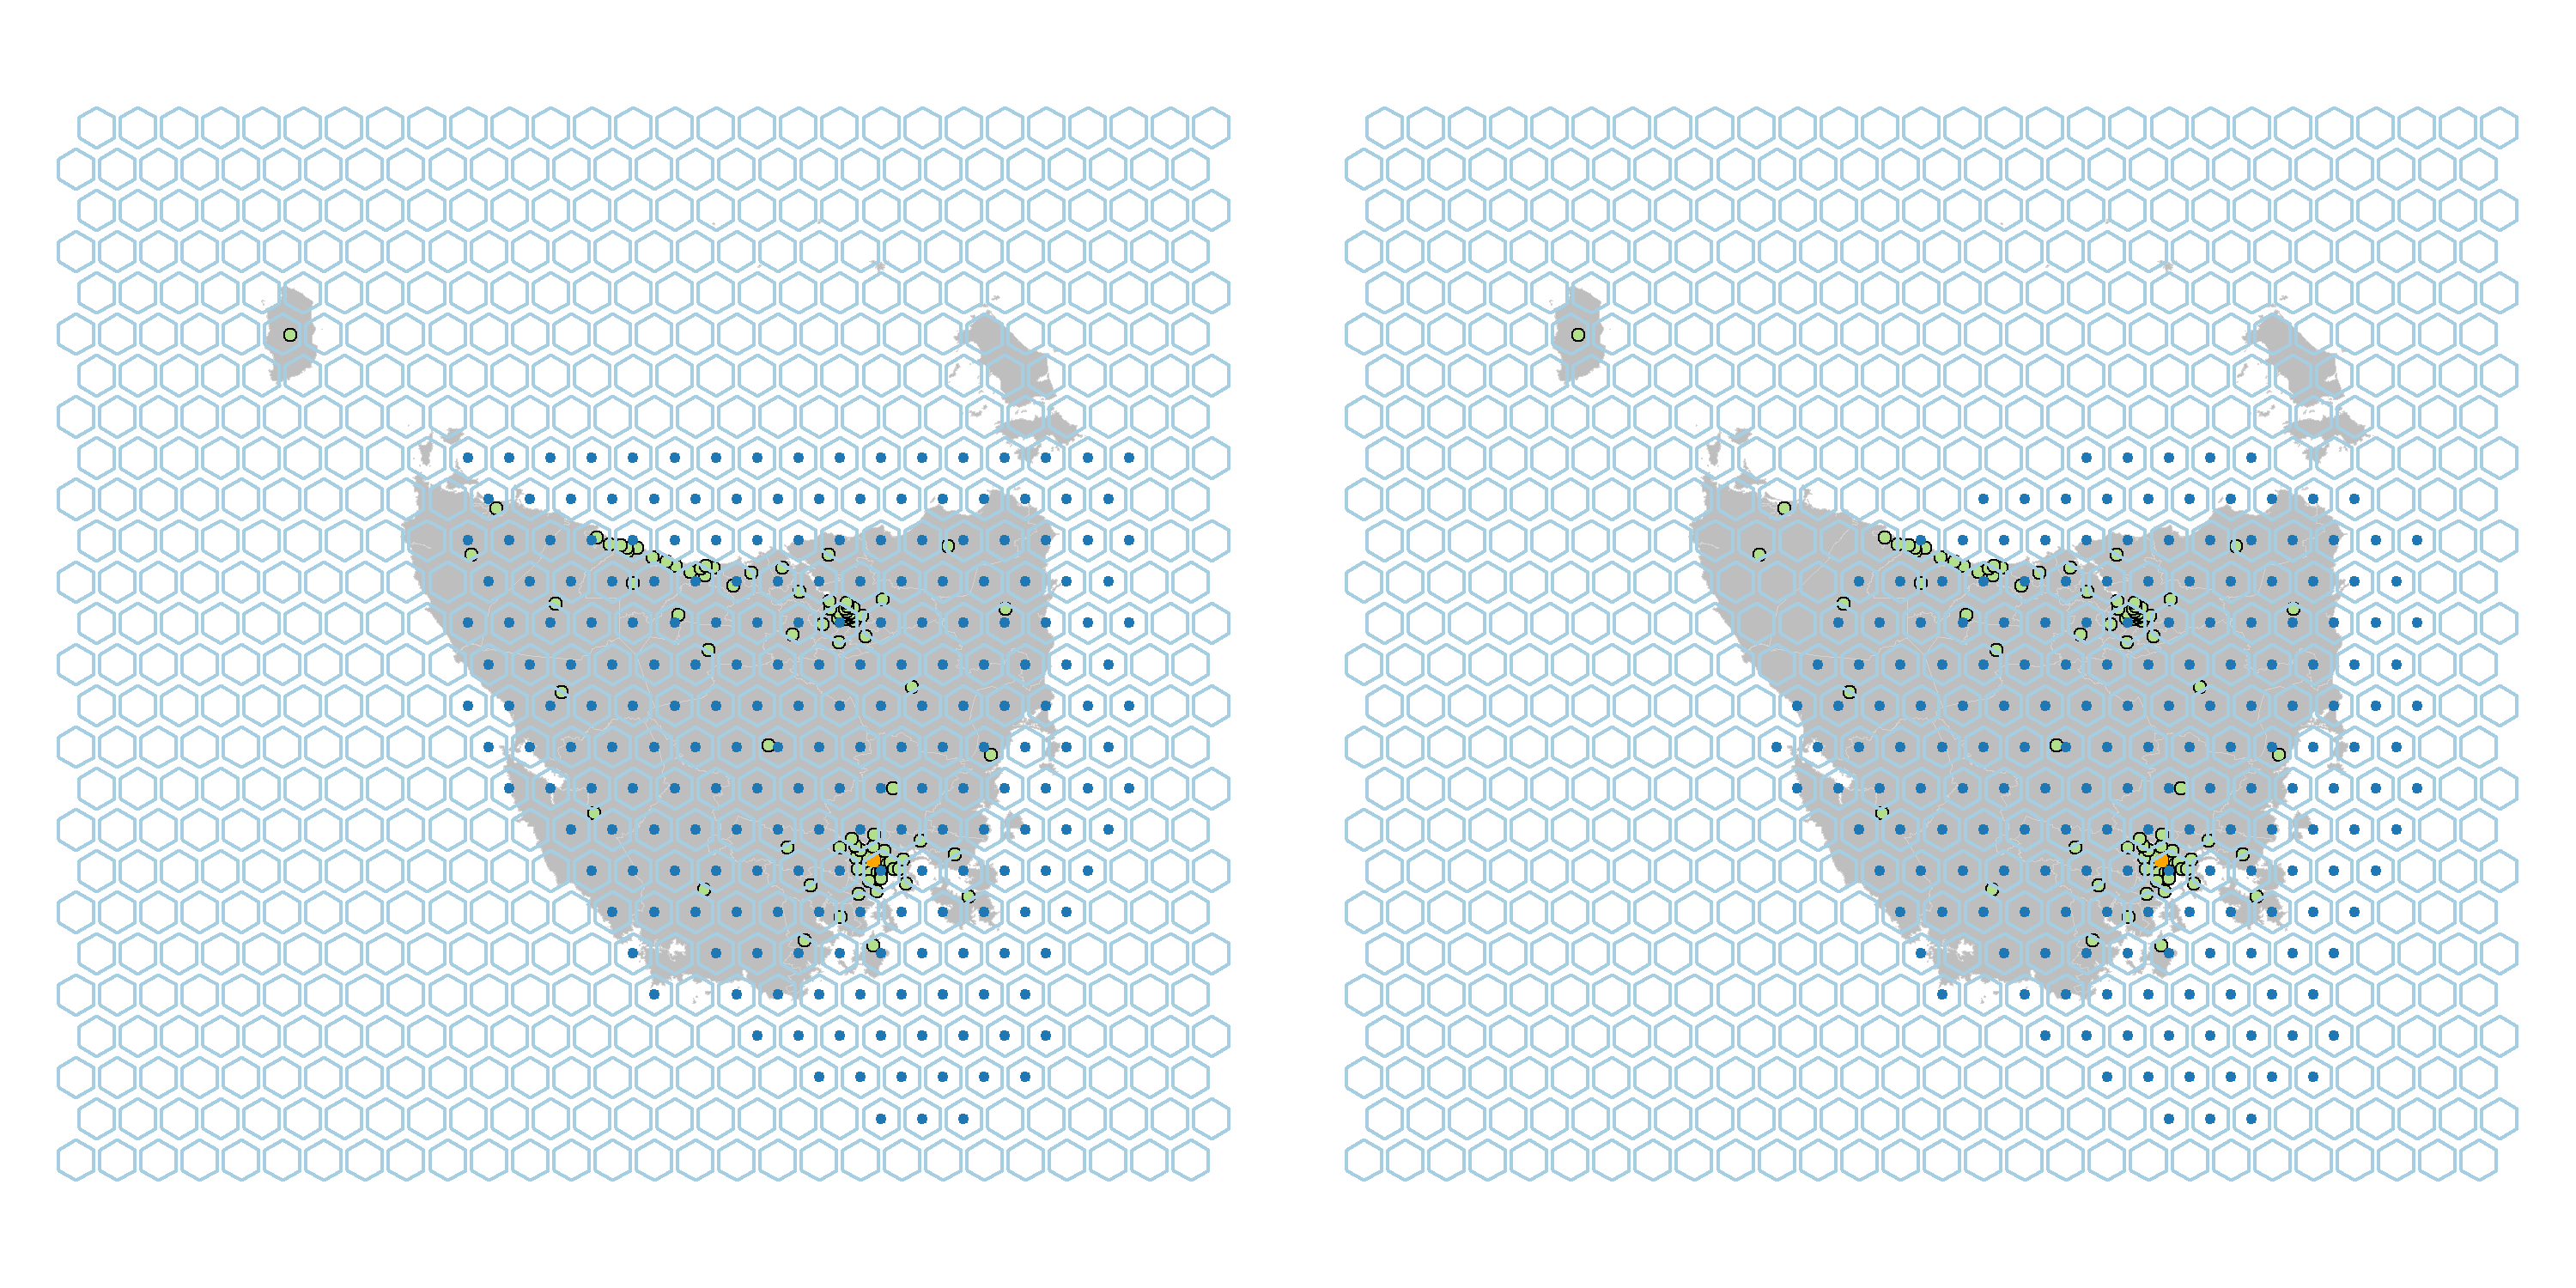
\includegraphics[width=1\linewidth]{figures/4grid} 

}

\caption[Filter for grid points within a square, then circular, distance for those closest to the centroid]{Filter for grid points within a square, then circular, distance for those closest to the centroid.}\label{fig:buffers}
\end{figure}
\end{CodeChunk}

The \code{width} parameter is used to take a slice of the remaining
points. The width is the amount of degrees used on either side of the
angle from the focal point to centroid location. This uses the angle
from the closest capital city, to the current centroid as seen in Figure
\ref{fig:angles} . This allows the spatial relationship to be preserved,
even when it is allocated to a hexagon that is further from the focal
point then the original centroid location.

\begin{CodeChunk}
\begin{figure}

{\centering 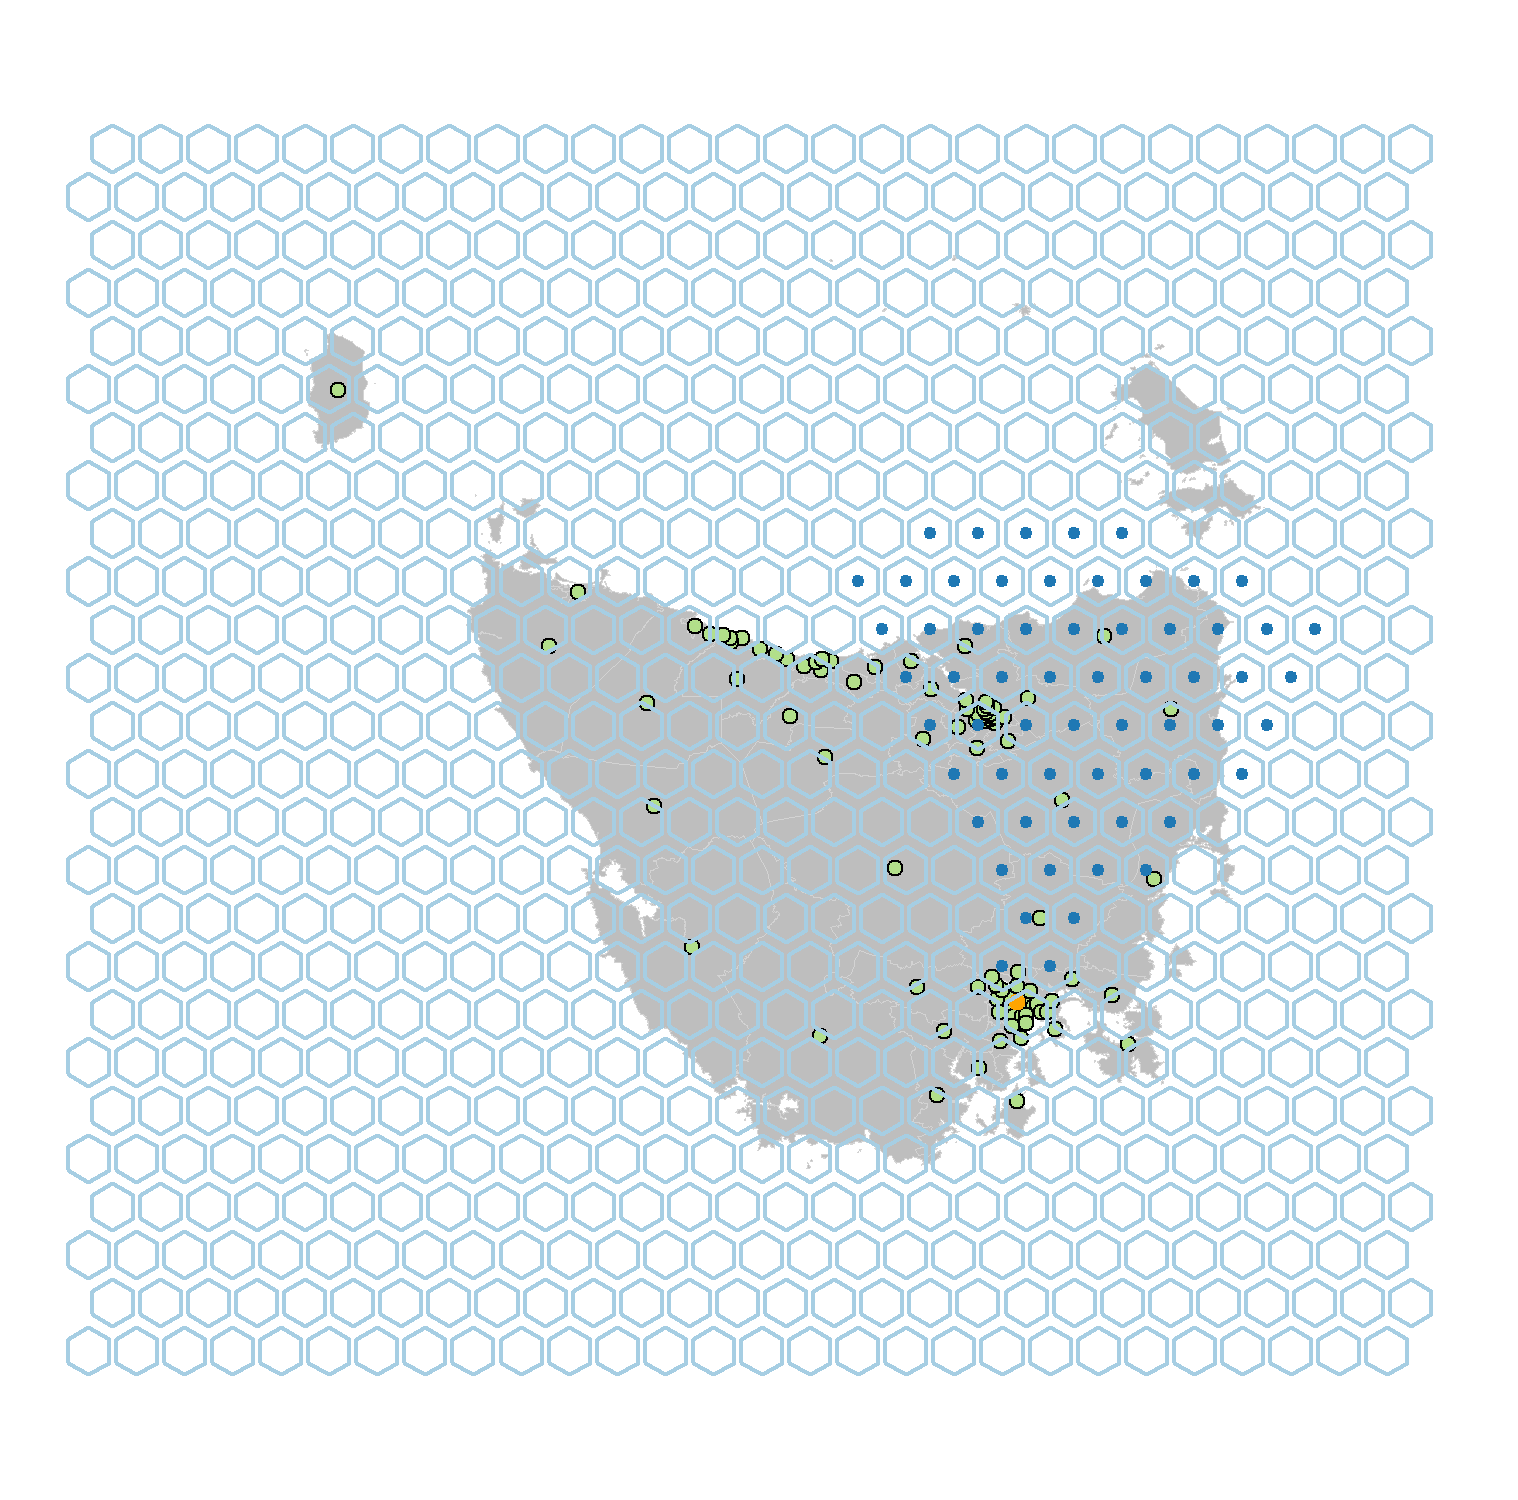
\includegraphics[width=1\linewidth]{figures/5allocate} 

}

\caption[Filter for grid points within the angle from the focal point to the centroid]{Filter for grid points within the angle from the focal point to the centroid.}\label{fig:angles}
\end{figure}
\end{CodeChunk}

If no available hexagon grid point is found within the original filter
distance and angle, the distance is expanded, only when a maximum
distance is reached will the angle expand to accommodate more possible
grid points.\\
By default the angle filter to hexagon grid points that fall within the
bounds of the angle from the focal point to the geographic centroid,
plus and minus 30 degrees. This will increase if no points can be found
within the \code{hex_filter} distance. The default angle of 30 was
chosen to allow the algorithm to choose hexagons that best maintained
the spatial relationship between the focal point and geographic
centroid.

\begin{CodeChunk}
\begin{figure}

{\centering 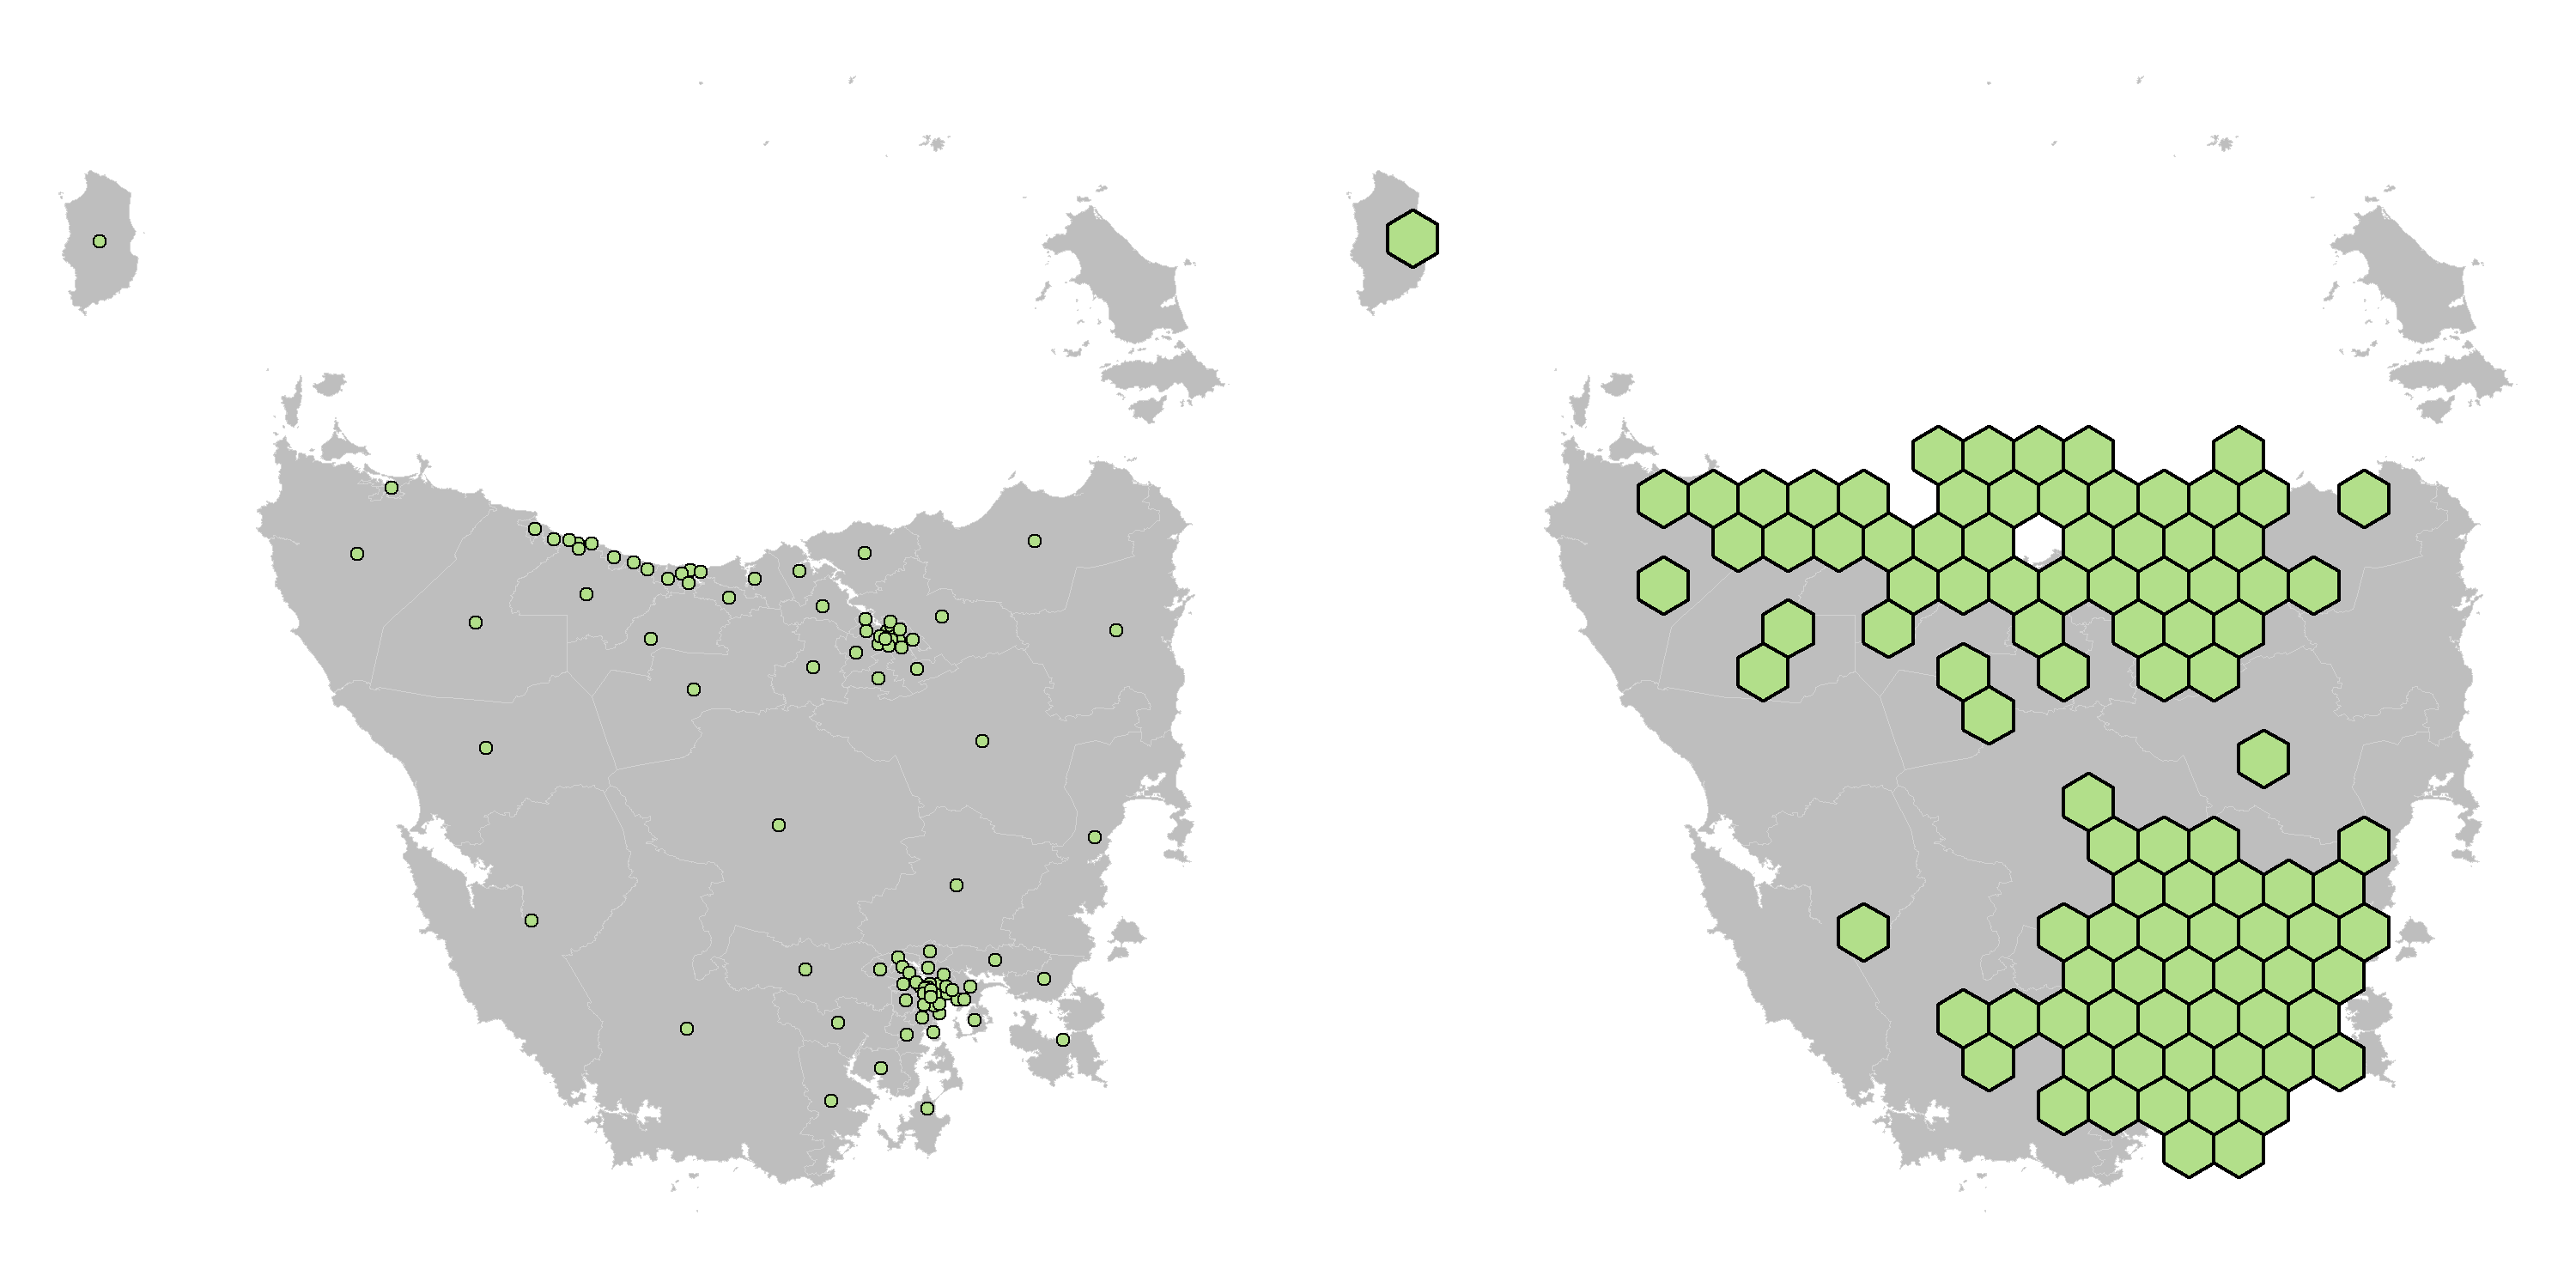
\includegraphics[width=1\linewidth]{figures/6allocate} 

}

\caption[A complete hexagon tile map of Tasmania]{A complete hexagon tile map of Tasmania.}\label{fig:buffs}
\end{figure}
\end{CodeChunk}

A complete hexagon tile map of Tasmania is created by applying the
algorithm steps to each centroid. The hexagon tile map visualisation is
used below to visualise the Australian Cancer Atlas data. Two views of
the same data are produced by filling according to the Lung Cancer
Standardised Incidence Rates (SIRs) downloaded from the Australian
Cancer Atlas site. This small example in Figure \ref{fig:sir} shows the
group of blue areas in the Hobart CBD more prominently in the hexagon
tile map (b). The small red areas visible in the choropleth map (a)
along the north coast are much larger in the hexagon tile maps. The
hexagon tile map shows less yellow, this no longer overwhelms the map
space with the information regarding the rural areas.

\begin{CodeChunk}
\begin{figure}

{\centering 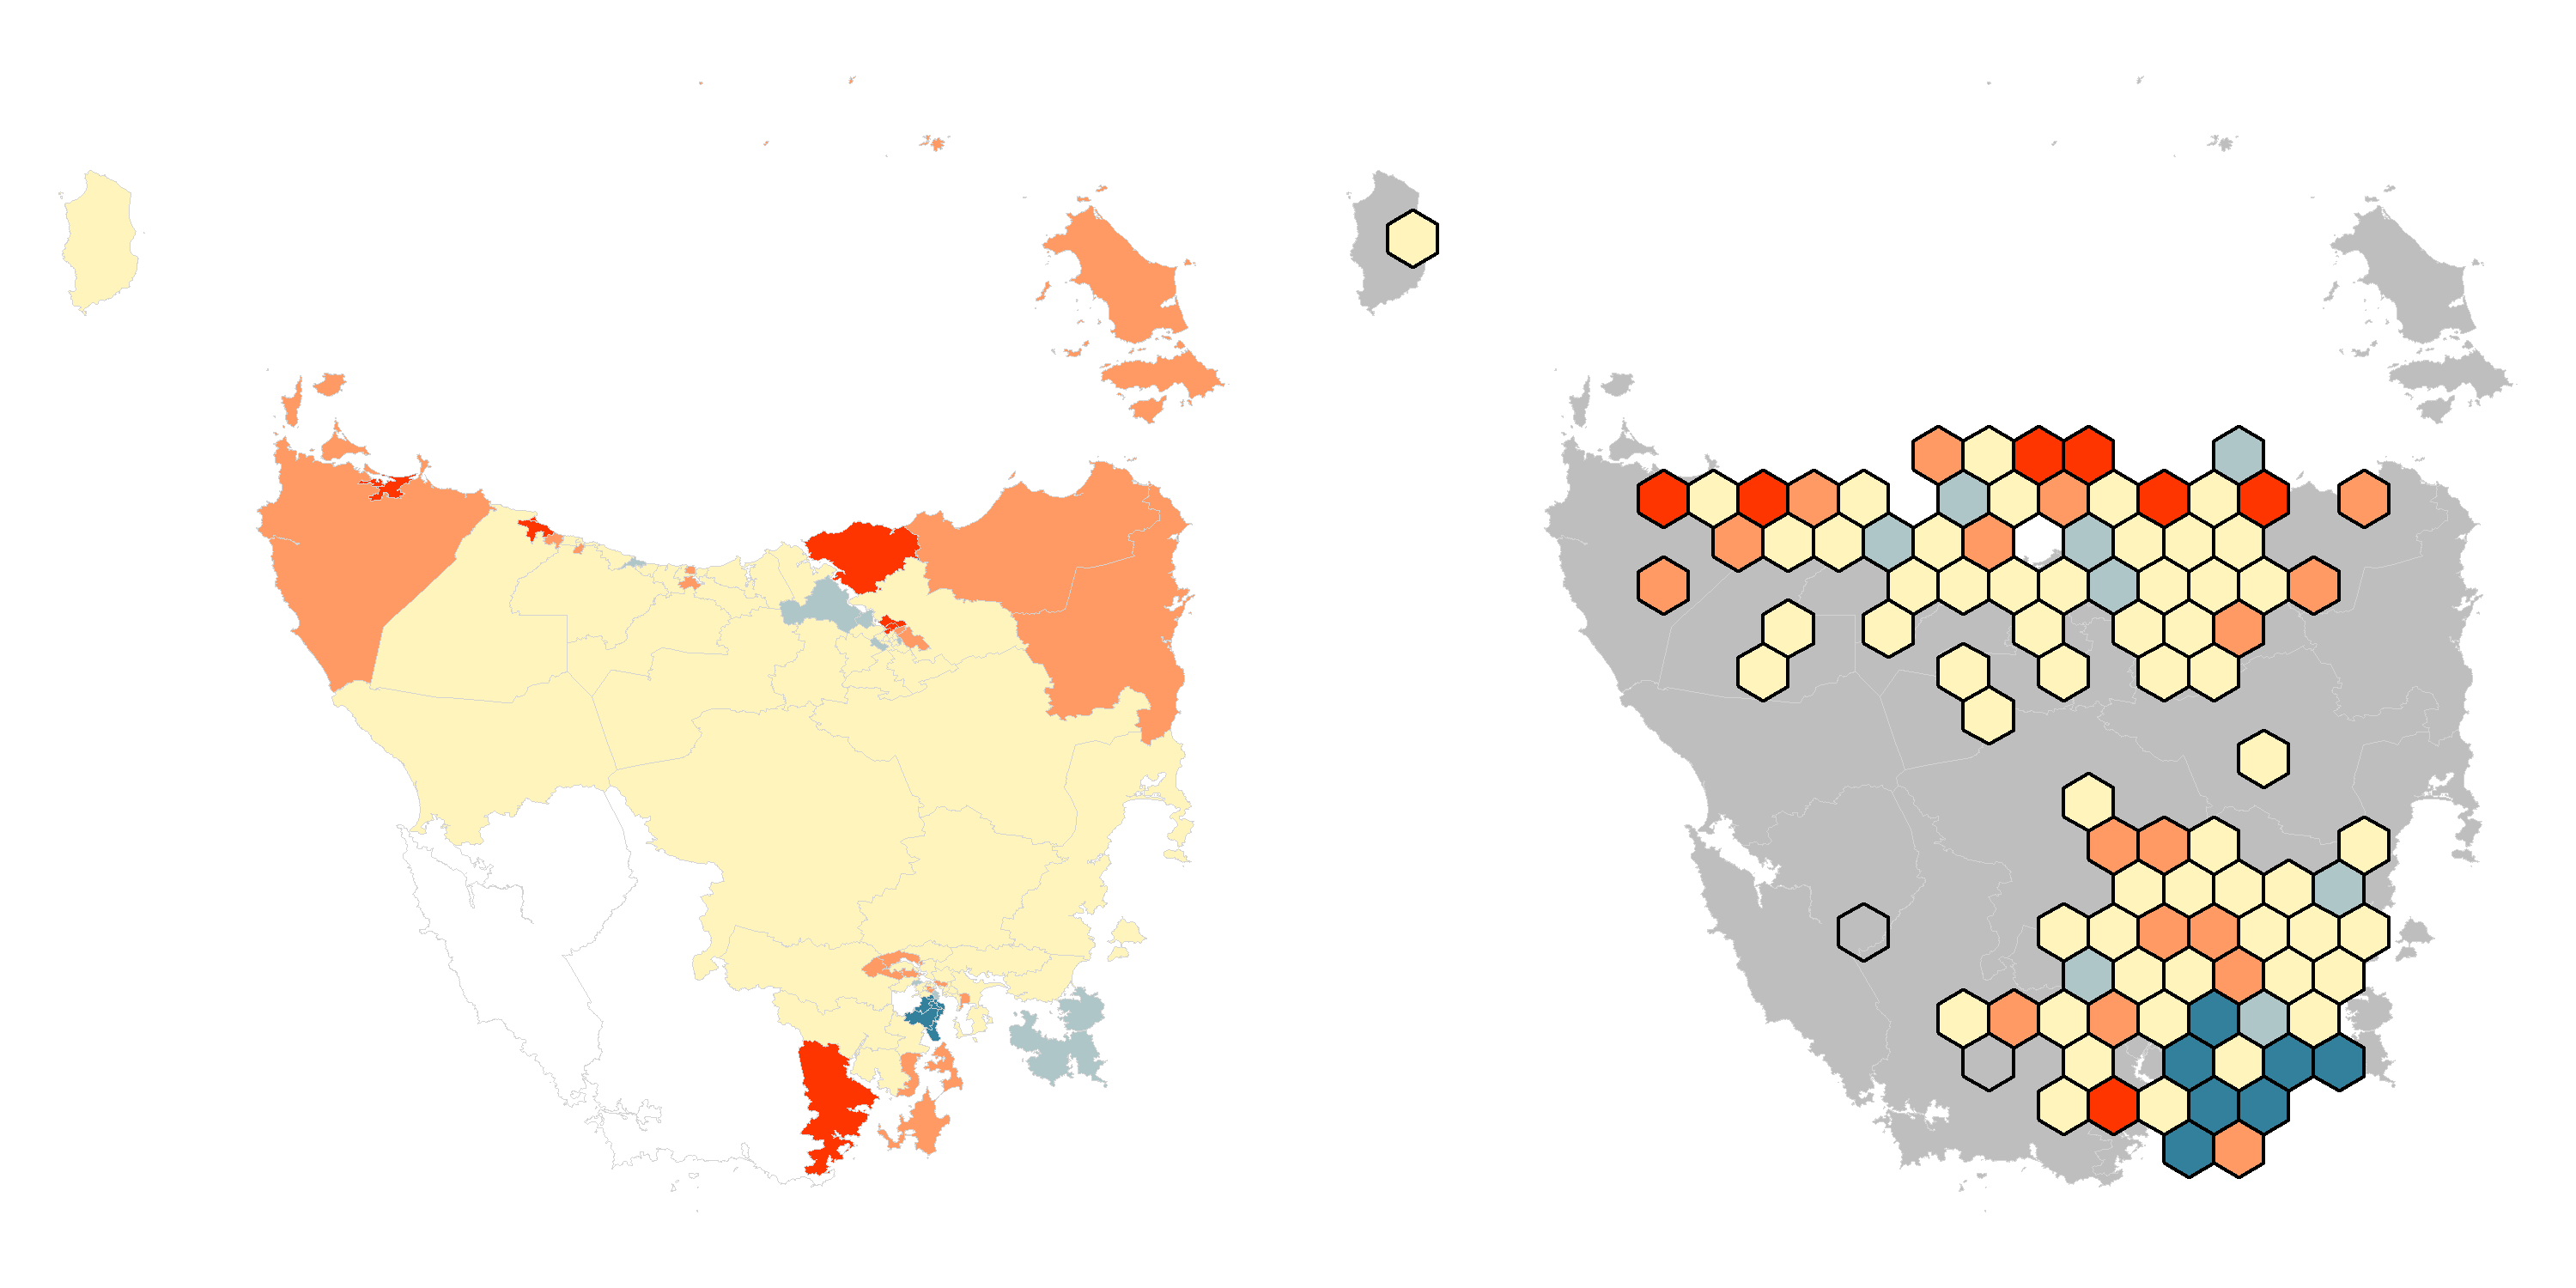
\includegraphics[width=1\linewidth]{figures/7SIR} 

}

\caption[The Australian Cancer Atlas data has determined the colour of each Statistical Area of Australian at Level 2]{The Australian Cancer Atlas data has determined the colour of each Statistical Area of Australian at Level 2. A choropleth map (a) of Standardised Incidence Rates (SIRs) is paired with a hexagon tile map (b) to contrast the colours that are made obvious when every SA2 is equally represented.}\label{fig:sir}
\end{figure}
\end{CodeChunk}

\hypertarget{neighbour-relationships}{%
\subsection{Neighbour relationships}\label{neighbour-relationships}}

It is possible to consider the neighbouring areas for each SA2, for
stronger preservation of the spatial distribution.

An additional step can be included to allow the neighbours that have
alredy been allocated to influence the placement of the current
centroid. This requires specifying the \code{sf} object as the argument
for the \code{use_neighbours} parameter. This calculates neighbours
using intersections of their polygons. This occurs for all areas before
any allocations begin.

During the allocation of each centroid, the list of neighbours is
consulted. If any neighbour was already allocated, the hexagons
surrounding the neighbours on the grid are prioritised. For multiple
neighbours, the neighbouring hexagon grid points are aggregated and
considered in order of distance from the original centroid.

\hypertarget{using-sugarbag}{%
\section{Using sugarbag}\label{using-sugarbag}}

\hypertarget{installation}{%
\subsection{Installation}\label{installation}}

The package can be installed from CRAN:

\begin{CodeChunk}

\begin{CodeInput}
R> install.packages("sugarbag")
\end{CodeInput}
\end{CodeChunk}

and the development version can be install from the GitHub repository:

\begin{CodeChunk}

\begin{CodeInput}
R> devtools::install_github("srkobakian","sugarbag")
\end{CodeInput}
\end{CodeChunk}

Load the library into your R session with:

\begin{CodeChunk}

\begin{CodeInput}
R> library(sugarbag)
\end{CodeInput}
\end{CodeChunk}

\hypertarget{creating-a-hexagon-tile-map}{%
\subsection{Creating a hexagon tile
map}\label{creating-a-hexagon-tile-map}}

The following code creates the hexagon tile map for all the Statistical
Areas at Level 2 in Tasmania.

\begin{CodeChunk}

\begin{CodeInput}
R> # Load data
R> data(tas_sa2)
R> 
R> # Create centroids set
R> centroids <- create_centroids(tas_sa2, "SA2_NAME16")
R> 
R> # Create hexagon grid
R> grid <- create_grid(centroids = centroids,
R>     hex_size = 0.2,
R>     buffer_dist = 1.2)
R> 
R> # Allocate polygon centroids to hexagon grid points
R> hex_allocated <- allocate(
R>   centroids = centroids,
R>   hex_grid = grid,
R>   sf_id = "SA2_NAME16",
R>   # same column used in create_centroids
R>   hex_size = 0.2,
R>   # same size used in create_grid
R>   hex_filter = 10,
R>   use_neighbours = tas_sa2,
R>   focal_points = capital_cities %>% filter(points == "Hobart"),
R>   width = 35,
R>   verbose = FALSE)
R> 
R> # Prepare to plot
R> fort_hex <- fortify_hexagon(data = hex_allocated, sf_id = "SA2_NAME16", hex_size = 0.2)
R> 
R> # Make a plot
R> library(ggplot2)
R> ggplot(fort_hex) + 
R>   geom_polygon(aes(x=long, y=lat, group=hex_id, fill = lat)) +
R>   scale_fill_distiller("", palette="PRGn")
\end{CodeInput}
\end{CodeChunk}

\hypertarget{applications}{%
\section{Applications}\label{applications}}

\hypertarget{australian-cancer-atlas}{%
\subsection{Australian Cancer Atlas}\label{australian-cancer-atlas}}

The Australian Cancer Atlas \citep{TACA} allows estimates derived from
the models of Standardised Incidence Rates and excess deaths to be
downloaded. Figure \ref{fig:melanoma-geo} is a choropleth map that uses
colour to display the estimated Standardised Incidence Rate of melanoma
cancer for all persons for each SA2. The Australian choropleth map
display draws attention to the expanse of light blue areas across the
rural communities in all states. The SA2s around Brisbane stand out as
more orange and red. Comparatively, the hexagon tile map display in
Figure \ref{fig:melanoma-hex} draws attention to contrast of the blue
areas in Sydney and Melbourne and the capital city of Brisbane. In both
Sydney and Melbourne, the hexagons that represent the SA2 areas in the
inner-city areas have lower than average Incidence Rates.

With careful consideration of the choropleth map, the small geographic
inner city areas may have been noticed by viewers, but the hexagon tile
map display emphasises them. The communities in northern Queensland and
the Northern territory do not draw attention because of their size as in
the choropleth, but their colour is still noticably below average when
contrasted with the heaxgons further south.

To create this choropleth map the SA2 polygons for 2011 from the ABS.
The Standardised Incidence Ratios for each geographic unit are joined to
the appropriate polygons.

\begin{figure}

{\centering 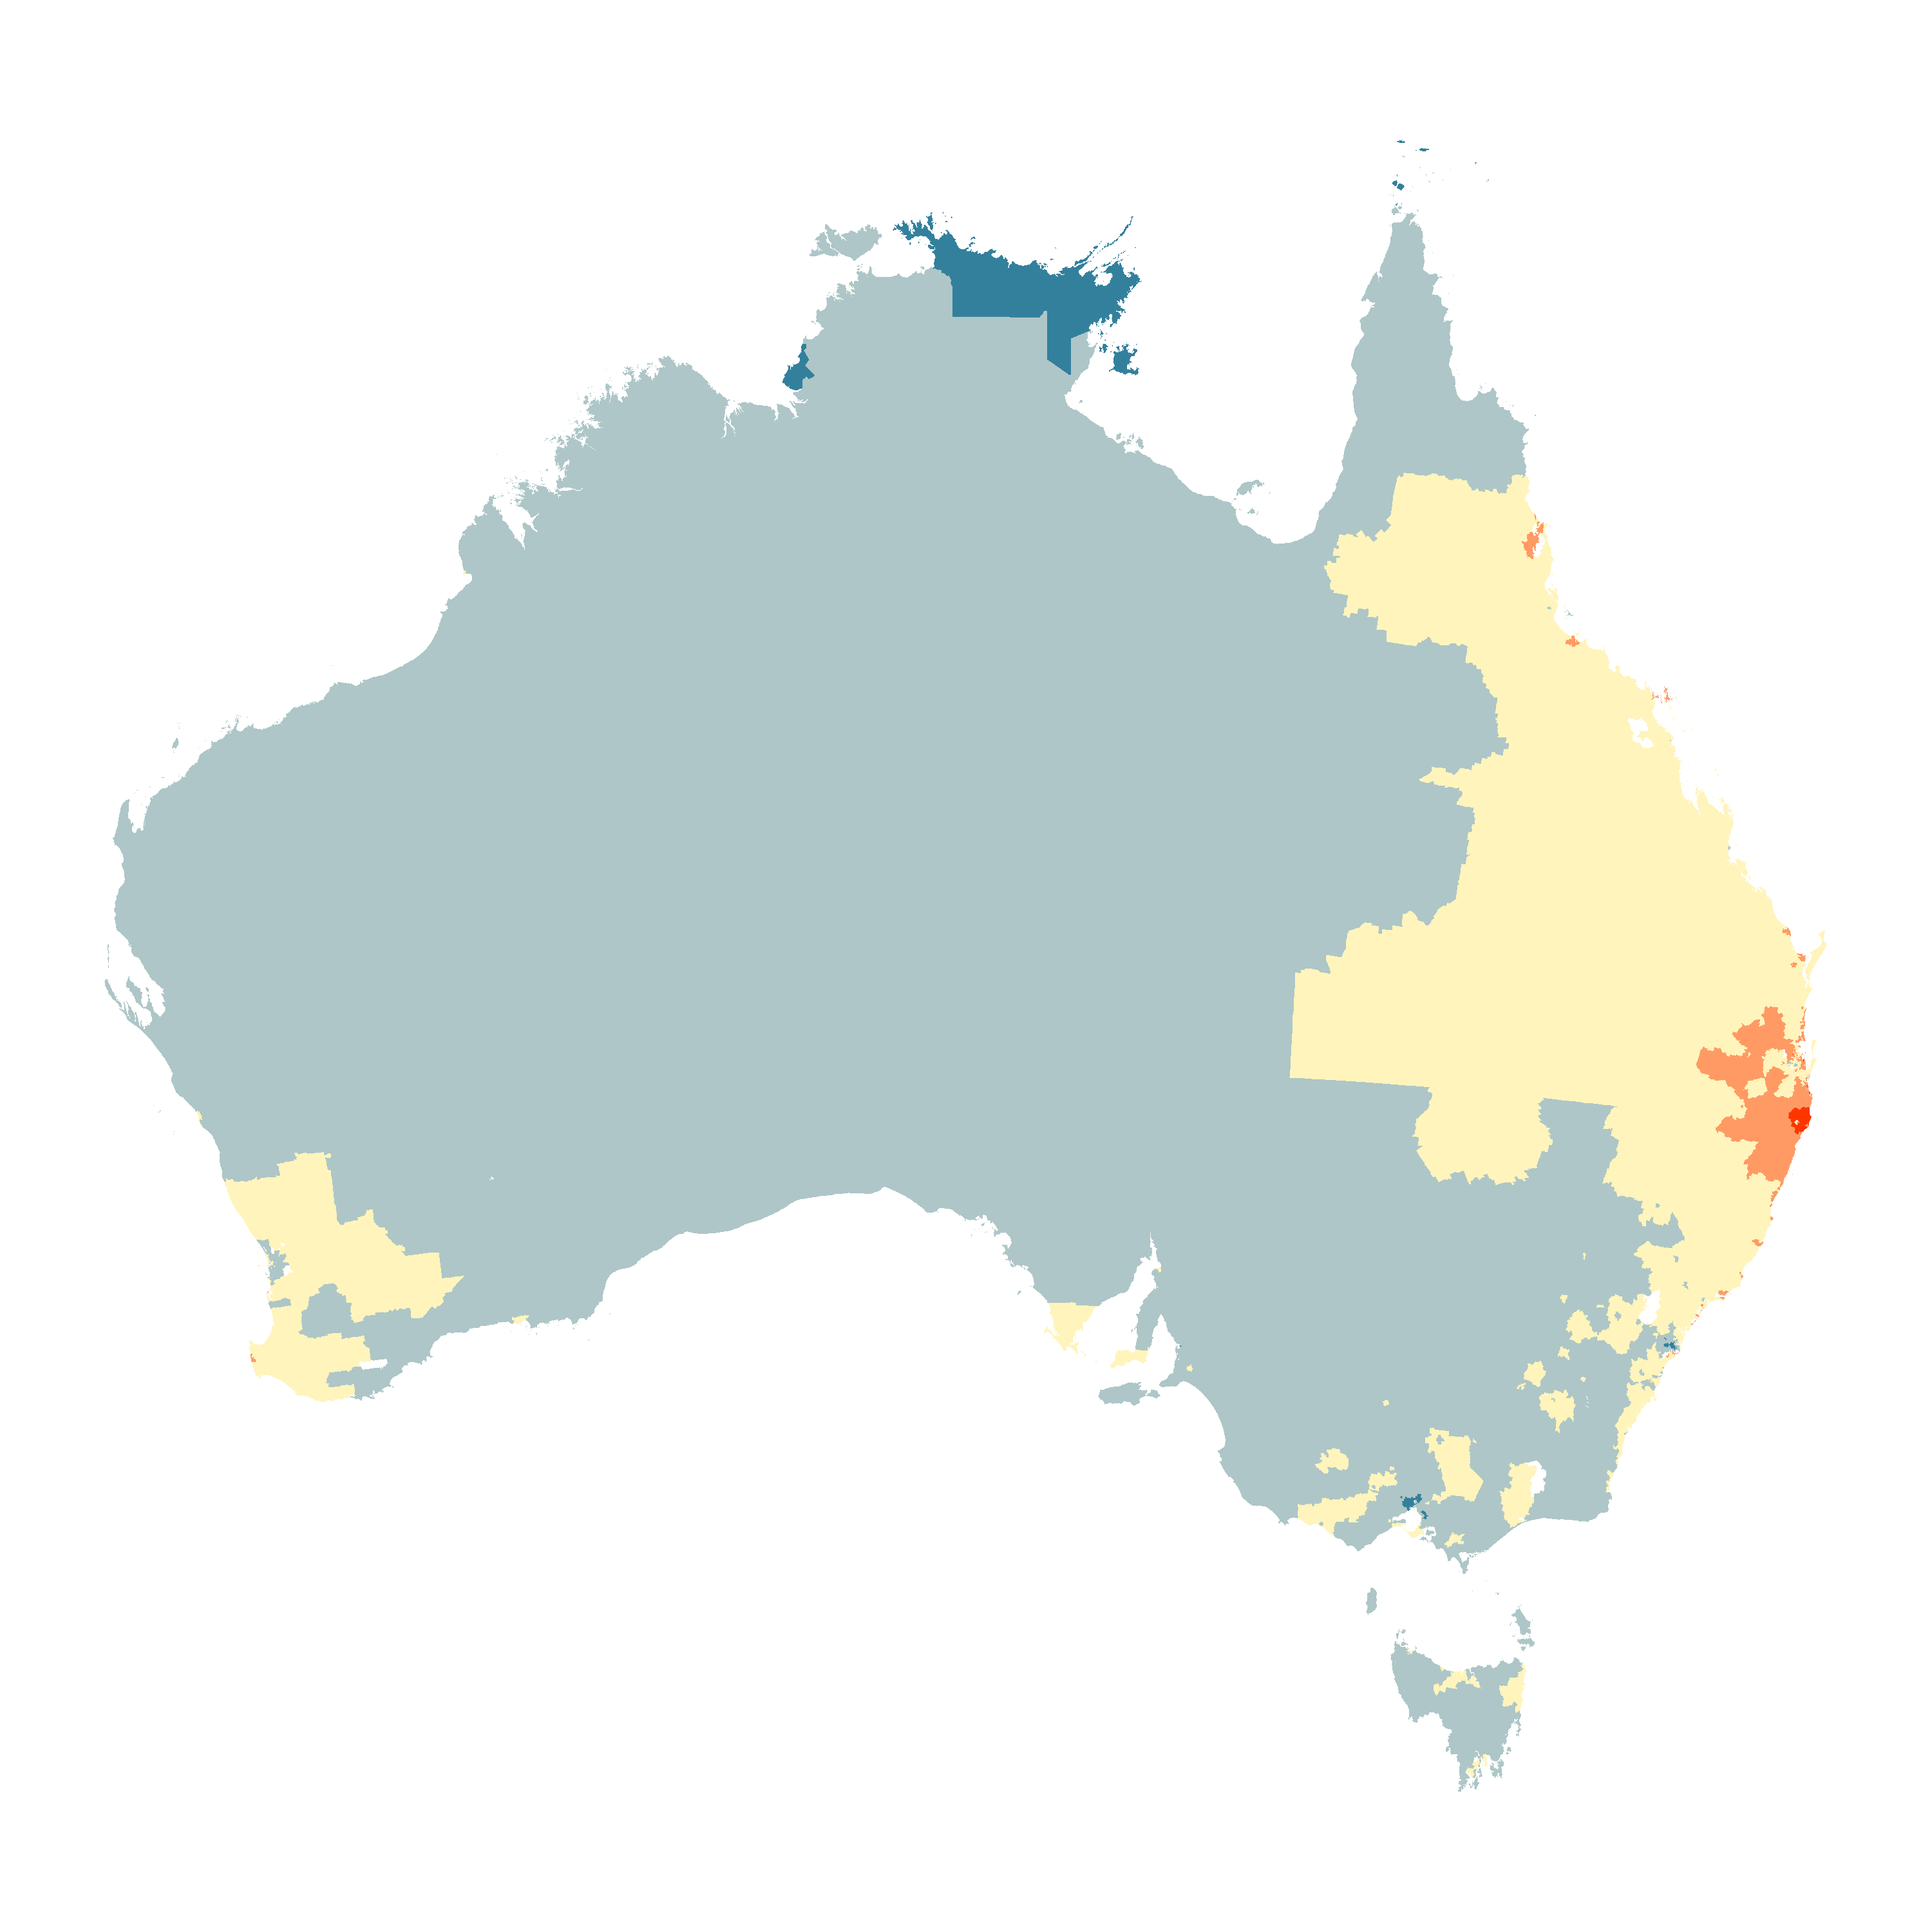
\includegraphics[width=0.6\linewidth]{figures/aus_melanoma_p} 

}

\caption[A choropleth map of the Statistical Areas of Australia at Level 2]{A choropleth map of the Statistical Areas of Australia at Level 2. The colours communicate the value of the estimated Standardised Incidence Rate of Melanoma for all persons, they range from much lower than average (blue) to much higher than average (red)}\label{fig:melanoma-geo}
\end{figure}

To create the hexagon tile map display, the same steps are followed as
outlined above:

\begin{itemize}
\tightlist
\item
  Create the set of centroid points
\item
  Create the hexagon grid points
\item
  Allocate each centroid to a hexagon grid point
\end{itemize}

\begin{figure}

{\centering 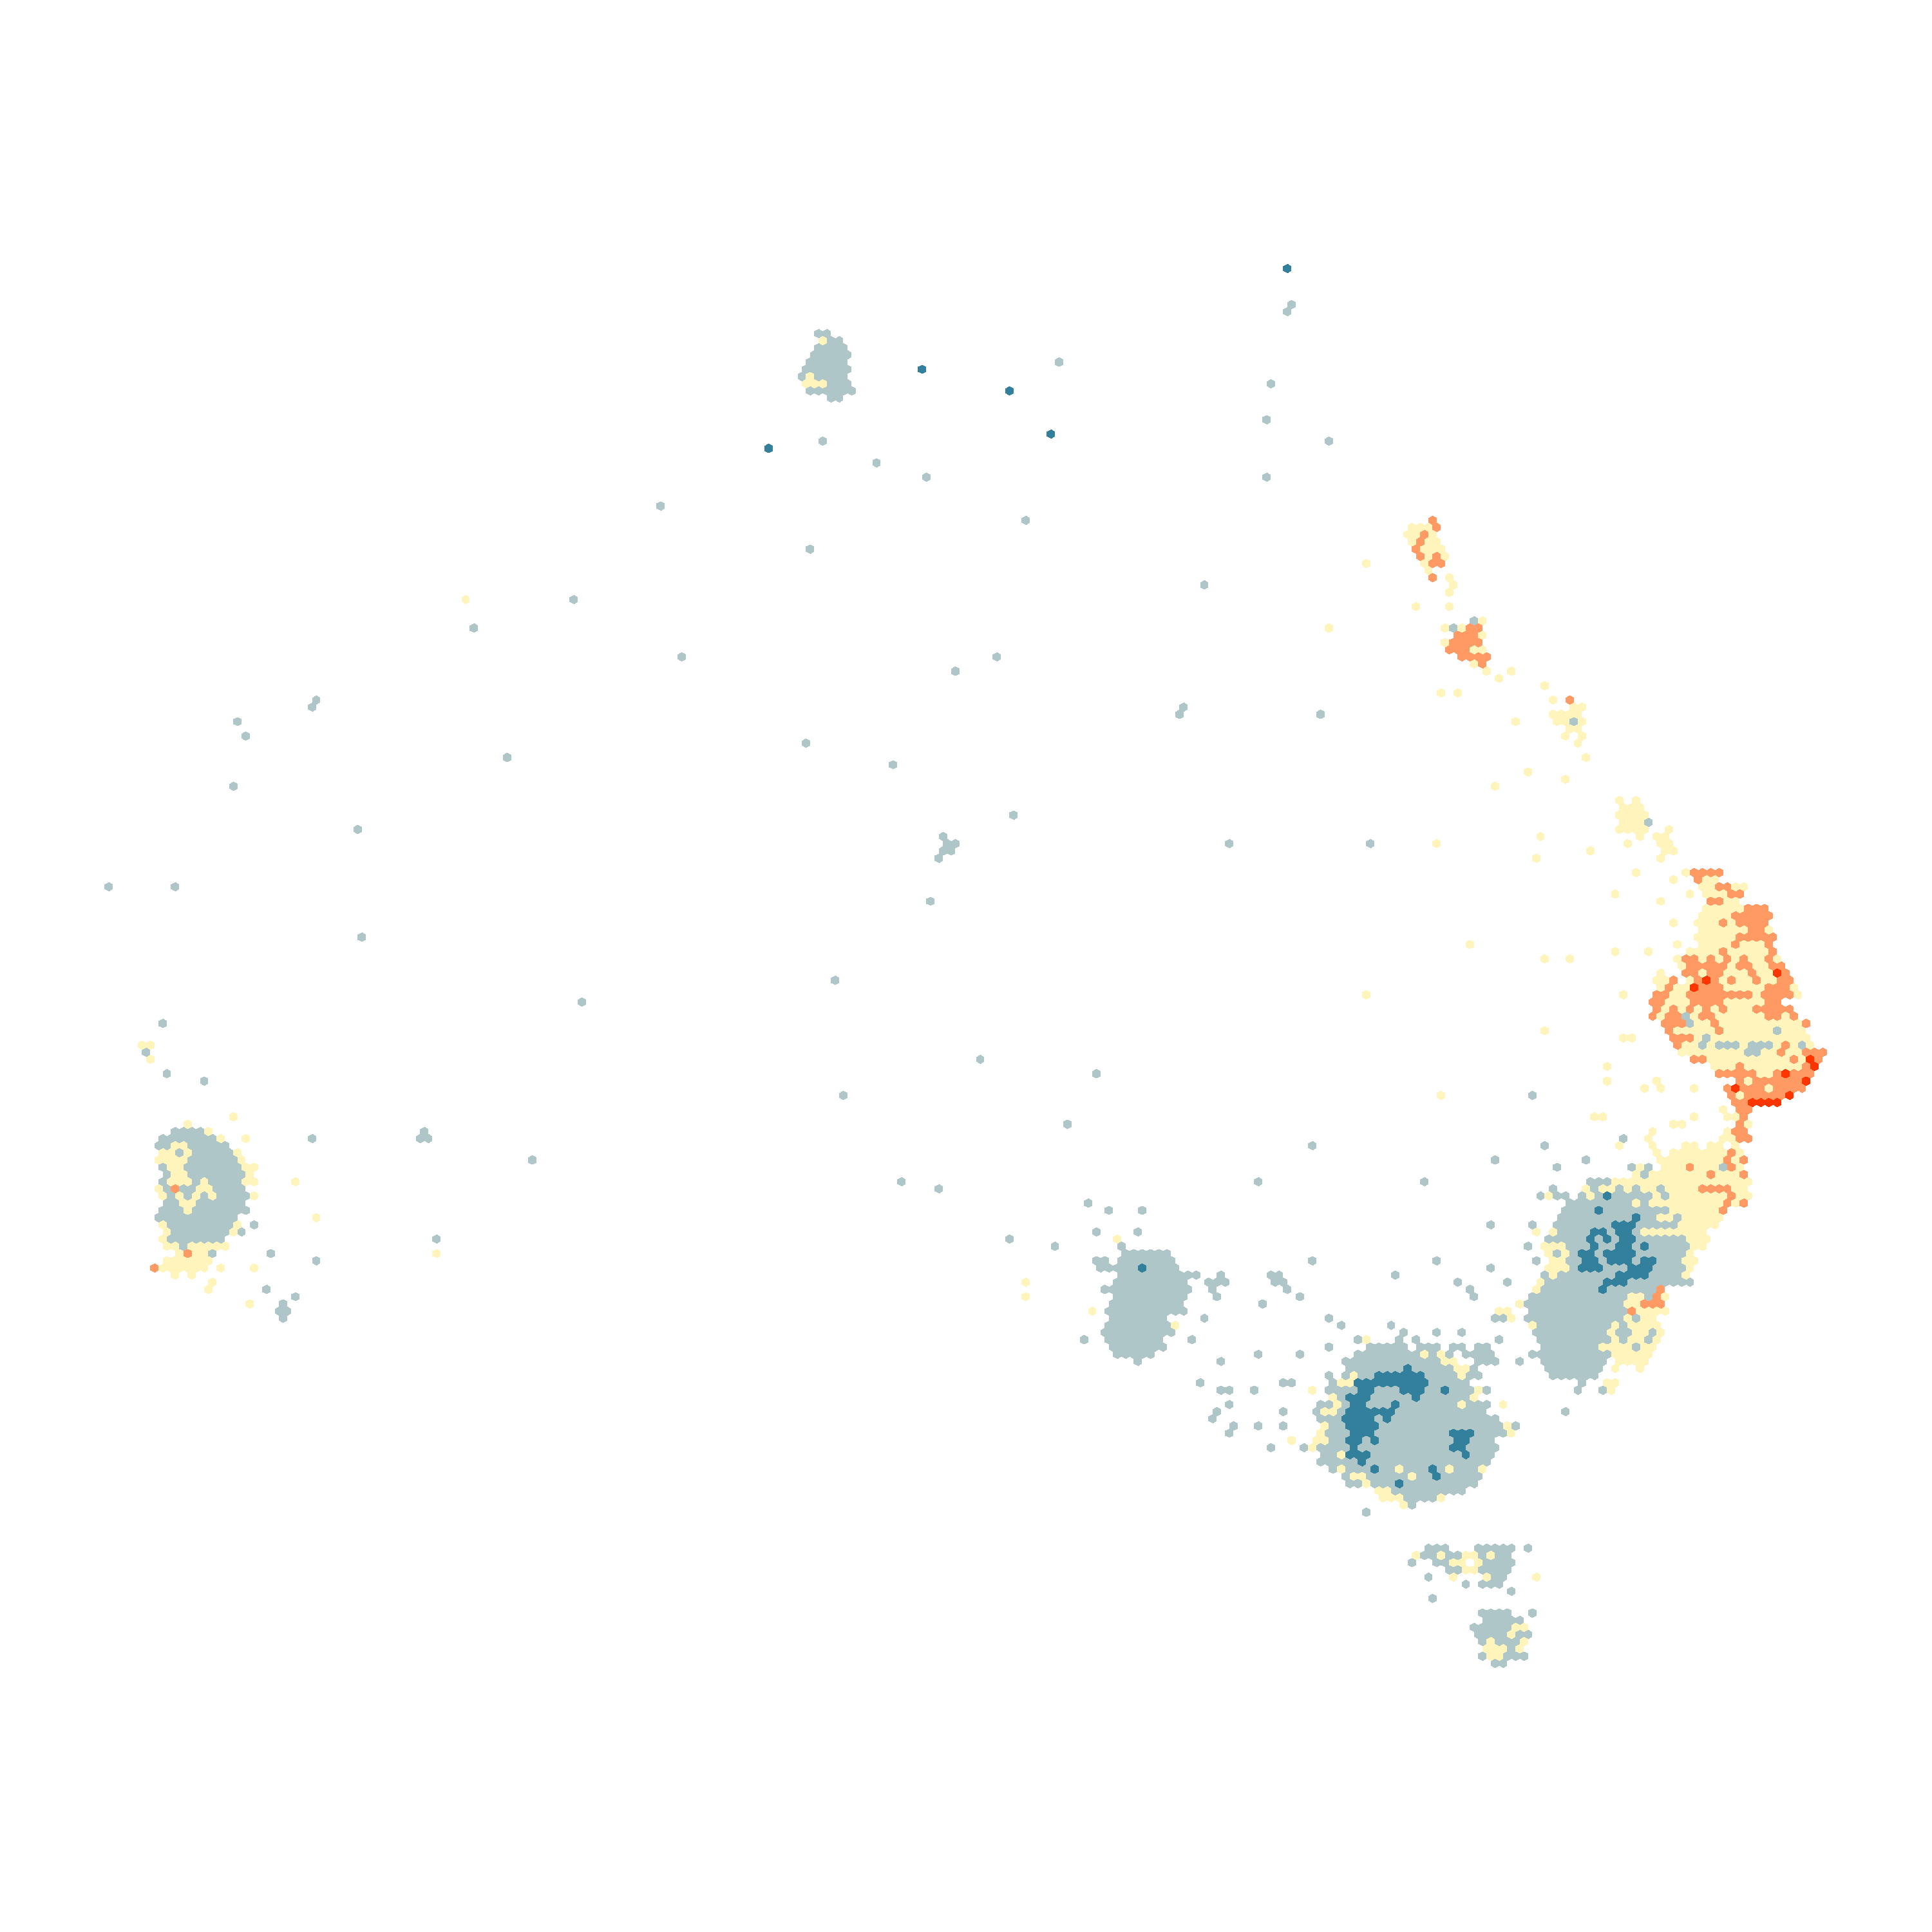
\includegraphics[width=0.6\linewidth]{figures/aus_melanoma_p_hex} 

}

\caption[A hexagon tile map of the Statistical Areas of Australia at Level 2]{A hexagon tile map of the Statistical Areas of Australia at Level 2. The colours communicate the value of the estimated Standardised Incidence Rate, they range from much lower than average (blue) to much higher than average (red)}\label{fig:melanoma-hex}
\end{figure}

\hypertarget{animation}{%
\section{Animation}\label{animation}}

The \pkg{gganimate} package can be used to make an animation. It
requires connecting the polygons for each area in two displays, which
can be done using the \code{sf_id} variable, such as the SA2 name. The
animation\footnote{This animation can be viewed at:
  \url{https://sugarbagjss.netlify.com/}} connecting these two displays
will highlight the rapid growth of the inner-city areas, and will
decrease the large rural areas. The hexagons that move the furthest will
move rapidly in the animation.

\hypertarget{conclusion}{%
\section{Conclusion}\label{conclusion}}

It is possible to use alternative maps to communicate spatial
distributions.While a choropleth map display is the current practice
spatial visualisation of geographical data. Current methods do not
always work for Australia due to the large geographic space between the
densely populated capital cities. The administrative boundaries may also
distract from the statistics communicated using colour.

Alternative maps highlight the value of the statistics across the
geographic units. Alternative mapping methods allow increased
understanding of the spatial distribution of a variable across the
population, by fairly representing each administrative area. This
acknowledges that the amount of residents can be different but
recognises that each population area is equally important. The solution
to this visualisation problem has equally sized areas, with
neighbourhood boundary connections. This map algorithm is implemented in
the \pkg{sugarbag} \citet{sugarbag} package written for \code{R}
\citet{R}. The \pkg{sugarbag} package creates tesselated hexagon tile
maps. The Australian application preserves the spatial relationships,
emphasising capital cities. The hexagon tile map is a visualisation
solution that highlights spatial distributions.

These hexagons equally represent each area. However, the tesselation
does not allow the size of the hexagons to represent another variable,
similar to the choropleth maps. The algorithm is heavily dependent on
the focal points used, as this determines the order of allocation. It
works on the assumption that viewers can use directional relationships
to identify their neighbourhoods but this can be aided by the animation.

Future work will include refining the algorithm. It would be possible to
take a logarithmic function rather than a direct angle to help choose a
closer hexagon to the original centroid location, before increasing the
width of the angle used to filter the hexagons.

This algorithm has only been tested using single countries, and does not
consider definite borders of countries. While the buffer allows
extention beyond the furthest centroids, there is no mechanism to
protect the borders and ensure centroids are placed within the
geographic borders of a country.

This algorithm is an effective start to creating hexagon tile maps for
many geographic units.

\hypertarget{acknowledgements}{%
\section{Acknowledgements}\label{acknowledgements}}

The authors would like to thank the Australian Cancer Atlas team for
discussions regarding alternative spatial visualizations. They would
also like to thank Professor Kerrie Mengersen for suggestions and
comments. Mitchell O'Hara-Wild provided assistance with some parts of
the algorithm and code. Sayani Gupta provided helpful advice on parts of
this paper.

The code for \pkg{sugarbag} \citep{sugarbag} can be found on
\href{https://cran.r-project.org/web/packages/sugarbag/index.html}{CRAN},
along with vignettes on installation and usage.

\bibliography{sugarbag.bib}


\end{document}

